% =====================================================================
%  Smart Energy Grid Analytics - Assignment I report (Overleaf)
%  Compiler: pdfLaTeX.  Upload the whole "report" folder to Overleaf.
%  Screenshots: put PNG files in screenshots/ with the names used in
%  the \shot{...} commands; missing ones show as labelled placeholders.
% =====================================================================
\documentclass[11pt,a4paper]{article}
\usepackage[utf8]{inputenc}
\usepackage[T1]{fontenc}
\usepackage[margin=2.2cm]{geometry}
\usepackage{graphicx}
\usepackage{booktabs}
\usepackage{tabularx}
\usepackage{array}
\usepackage{float}
\usepackage{xcolor}
\usepackage{tcolorbox}
\usepackage{enumitem}
\usepackage{amsmath}
\usepackage{caption}
\usepackage{listings}
\usepackage{fancyhdr}
\usepackage[hidelinks]{hyperref}

\definecolor{teambg}{HTML}{FDF6E3}
\definecolor{teamframe}{HTML}{E8A06A}
\definecolor{teamtitle}{HTML}{A0582A}
\definecolor{codebg}{HTML}{F6F8FA}

\newcommand{\submissiondate}{15 October 2026}
\newcommand{\repourl}{\url{https://github.com/<your-account>/<repository>}}

\lstset{basicstyle=\ttfamily\footnotesize, backgroundcolor=\color{codebg},
        frame=single, rulecolor=\color{black!15}, breaklines=true,
        columns=fullflexible, keepspaces=true, showstringspaces=false}

\setlist{itemsep=2pt, topsep=4pt}
\captionsetup{font=small, labelfont=bf}
\renewcommand{\arraystretch}{1.15}

% \shot{file.png}{caption}: embeds screenshots/file.png, or a placeholder box
\newcommand{\shot}[2]{%
  \begin{figure}[H]\centering
  \IfFileExists{screenshots/#1}%
    {\includegraphics[width=0.92\linewidth]{screenshots/#1}}%
    {\fcolorbox{teamframe}{teambg}{\parbox[c][2.6cm][c]{0.88\linewidth}{\centering\small
      \textbf{Screenshot to insert:} \texttt{screenshots/\detokenize{#1}}\\[3pt]#2\\[2pt]
      \textit{(show the command, its result, the taskbar and the clock)}}}}%
  \caption{#2}
  \end{figure}}

\pagestyle{fancy}
\fancyhf{}
\lhead{\small Smart Energy Grid Analytics -- Assignment I}
\rhead{\small Mashami, Murenzi, Shami}
\cfoot{\small \thepage}

\begin{document}

% ------------------------------------------------------------------ title
\begin{titlepage}
\centering
\vspace*{2.5cm}
{\Huge\bfseries Smart Energy Grid Analytics\par}
\vspace{0.4cm}
{\Large Advanced Big Data Analytics -- Assignment I\par}
\vspace{0.3cm}
{\large Ingestion, storage benchmarking, analysis, dashboards and forecasting\\
for 4,000 smart meters\par}
\vspace{2.2cm}

\begin{tcolorbox}[colback=teambg, colframe=teamframe, boxrule=0.6pt, arc=0pt,
                  width=0.9\linewidth, halign=center, top=10pt, bottom=10pt]
{\large\bfseries\color{teamtitle} TEAM DETAILS}\\[8pt]
\begin{tabular}{ll}
101406 & Pacifique Mashami\\
101368 & Prince Murenzi\\
101371 & Delice Sebaganwa Shami\\
\end{tabular}\\[10pt]
Module: BIG DATA ESSENTIALS\\[6pt]
Instructor: KUNDAN KUMAR\\[6pt]
Date of Submission: \submissiondate
\end{tcolorbox}

\vfill
{\small Repository: \repourl}
\end{titlepage}

\tableofcontents
\newpage

% ================================================================== 0
\section*{Overview}
\addcontentsline{toc}{section}{Overview}
We acted as data analysts for an electricity utility. The supplied, unchanged
generator \texttt{smart\_meter\_simulator.py} (v3.0) produced 15-minute readings
from 4,000 meters for 1--28 September 2026. We built an MQTT and bulk ingestion
pipeline into PostgreSQL/TimescaleDB, investigated and cleaned the data,
benchmarked chunk intervals and compression strategies, analysed demand, built
continuous aggregates and two dashboards, and forecast next-day hourly regional
consumption. All times are CAT (Africa/Kigali, UTC+2). All code is our own except
the generator; the execution order is in the repository \texttt{README.md}.

\begin{table}[H]\centering\small
\begin{tabular}{lll}\toprule
Area & Choice & Result\\\midrule
Ingestion & generator $\rightarrow$ CSV $\rightarrow$ \texttt{COPY} & 10,696,848 rows in 194.6\,s\\
Storage & 1-day chunks, compressed, segmented by \texttt{meter\_id} & 64.6\,\% smaller\\
Dashboards & continuous aggregates & 6.7$\times$ faster refresh\\
Anomalies & same-meter, same-slot median ratio rule & 40/40 events, 0 false flags\\
Forecast & Ridge regression & MAE 4.56 vs 42.71\,kWh baseline\\\bottomrule
\end{tabular}
\caption{Summary of decisions and headline results.}
\end{table}

% ================================================================== 1
\section{Build the ingestion pipeline}

\subsection{Confirm the environment}
EMQX and PostgreSQL with TimescaleDB run as Docker containers
(\texttt{docker-compose.yml}). We created the database \texttt{energy\_grid},
enabled TimescaleDB and set
\texttt{ALTER DATABASE energy\_grid SET timezone TO 'Africa/Kigali'}, so every
session works in CAT. Daily buckets use
\texttt{time\_bucket('1 day', ts, 'Africa/Kigali')}, which aligns them to CAT
midnight. The details below were recorded by \texttt{src/s1\_1\_environment.py}.

\begin{table}[H]\centering\small
\begin{tabularx}{0.92\linewidth}{lX}\toprule
Item & Value\\\midrule
CPU & Apple M3, 8 cores\\
RAM & 16 GB\\
Operating system & macOS 14.6\\
Storage & SSD (Apple Fabric)\\
Python & 3.13.7\\
EMQX & 6.3.1\\
PostgreSQL & 17.11\\
TimescaleDB & 2.30.2\\
\texttt{shared\_buffers} & 1959 MB\\
\texttt{work\_mem} & 7837 kB\\
\texttt{max\_parallel\_workers\_per\_gather} & 4\\
\texttt{jit} & off\\
PostgreSQL runtime & Docker container (\texttt{timescale/timescaledb:latest-pg17}) inside the
Docker Desktop Linux VM. VM limit: 8 CPUs and 7.65 GiB RAM. No per-container CPU or RAM limit.\\
Session time zone & Africa/Kigali\\\bottomrule
\end{tabularx}
\caption{Environment.}
\end{table}

\shot{1_1_broker.png}{EMQX broker running (\texttt{docker ps} / EMQX dashboard).}
\shot{1_1_database.png}{Connection to \texttt{energy\_grid}, the TimescaleDB extension and the session time zone.}

\subsection{Create the database structures}
\texttt{sql/02\_tables.sql} creates three tables:
\begin{itemize}
\item \texttt{energy\_live}, a regular table for the pilot;
\item \texttt{energy\_readings}, a hypertable on \texttt{event\_time} with one-day chunks and no primary
key, so duplicates are allowed;
\item \texttt{meters}.
\end{itemize}
The hypertable is created without default indexes and receives two explicit B-tree
indexes, \texttt{(event\_time DESC)} and \texttt{(meter\_id, event\_time DESC)}, so the
same indexes can be reproduced on every later hypertable.
\texttt{src/s1\_2\_load\_meters.py} inserted the 4,000 \texttt{meter\_metadata()}
dictionaries, and the count query confirmed 4,000 rows.

\begin{table}[H]\centering\small
\begin{tabularx}{\linewidth}{llllX}\toprule
Table & Column & Type & Unit & Meaning\\\midrule
energy\_live, & meter\_id & BIGINT & -- & ten-digit meter identifier\\
energy\_readings & event\_time & TIMESTAMPTZ & CAT time & start of the 15-minute interval\\
 & received\_time & TIMESTAMPTZ & CAT time & simulated arrival (not insert time)\\
 & power\_kw & DOUBLE PRECISION & kW & average power over the interval\\
 & voltage\_v & DOUBLE PRECISION & V & voltage\\
 & current\_a & DOUBLE PRECISION & A & current (power factor 0.95)\\
 & frequency\_hz & DOUBLE PRECISION & Hz & grid frequency\\
 & energy\_kwh & DOUBLE PRECISION & kWh & interval energy $\approx$ power\_kw $\times$ 0.25\,h\\\midrule
meters & meter\_id & BIGINT (PK) & -- & meter identifier\\
 & region & TEXT & -- & Region 1--10 (400 meters each)\\
 & customer\_type & TEXT & -- & residential, commercial, industrial\\
 & base\_power\_kw & DOUBLE PRECISION & kW & typical power level of the meter\\
 & power\_factor & DOUBLE PRECISION & none & real/apparent power ratio (0.95)\\\bottomrule
\end{tabularx}
\caption{Data dictionary.}
\end{table}

\shot{1_2_tables.png}{Columns and types of the three tables, and the one-day chunk interval.}
\shot{1_2_meters.png}{Query confirming 4,000 rows in \texttt{meters}.}

\subsection{Capture and publish a pilot stream}
The publisher (\texttt{src/s1\_3\_publisher.py}) takes the first 2,000 generator
dictionaries and publishes each as JSON to \texttt{energy/meters/\{meter\_id\}} with QoS 1
and no retained messages. A message counts as acknowledged when the broker's PUBACK
triggers \texttt{on\_publish}. The subscriber (\texttt{src/s1\_3\_subscriber.py}) is
started first on an empty \texttt{energy\_live}. It subscribes to
\texttt{energy/meters/\#} at QoS 1 with a persistent session and inserts the eight
fields of each message.

\begin{table}[H]\centering\small
\begin{tabular}{lrr}\toprule
Stage & Run 1 (faulty) & Run 2 (fixed)\\\midrule
Dictionaries taken from the generator & 2,000 & 2,000\\
Messages acknowledged by the broker & 2,000 & 2,000\\
Messages received by the subscriber & \textbf{1,208} & 2,000\\
Rows committed in \texttt{energy\_live} & \textbf{1,208} & 2,000\\\bottomrule
\end{tabular}
\caption{Pilot counts. Deliberate generator duplicates count as separate messages:
the 2,000 rows contain 1,994 distinct pairs.}
\end{table}

\paragraph{Fault diagnosis.}
\begin{itemize}
\item \textbf{Size.} The first run lost 792 messages (39.6\,\%) between the broker
and the subscriber. Nothing was lost between the generator and the broker.
\item \textbf{Evidence.} The subscriber log showed no parse errors, no failed inserts
and no redeliveries. The broker metrics (\texttt{emqx ctl broker metrics}) reported
\texttt{delivery.dropped.queue\_full = 792}.
\item \textbf{Cause.} Version 1 inserted and committed each row inside the MQTT
\texttt{on\_message} callback, which blocks the client's network loop. The
subscriber therefore drained about 200 messages per second, while the publisher sent
all 2,000 in about 1.4\,s. EMQX holds at most 1,000 queued messages per session and
discards new ones once that queue is full, even at QoS 1.
\item \textbf{Fix.} The callback now only parses each message and places it on an
in-process queue; a separate writer thread inserts batches of 200 rows and commits.
The repeated pilot delivered 2,000 at every stage.
\end{itemize}

\shot{1_3_publisher.png}{Publisher completion with 2,000 acknowledged messages.}
\shot{1_3_subscriber.png}{Subscriber received count.}
\shot{1_3_database.png}{Stored count in \texttt{energy\_live} and sample rows.}
\shot{1_3_fault_metrics.png}{First run: EMQX \texttt{delivery.dropped.queue\_full = 792}.}

% ================================================================== 2
\section{Capture and prepare the historical dataset}

\subsection{Capture and load the complete stream}
\textbf{Route: generator $\rightarrow$ CSV file $\rightarrow$ \texttt{COPY FROM STDIN}}
(\texttt{src/s2\_1\_capture\_load.py}). Readings are written to the CSV one
dictionary at a time, with progress printed every million rows, so memory use stays
constant. The file is then streamed into the empty \texttt{energy\_readings} in 8\,MB
blocks inside a single transaction. \texttt{dataset\_info()} gave
\texttt{planned\_readings} = 10,752,000 and \texttt{emitted\_readings} = 10,696,848.

\begin{table}[H]\centering\small
\begin{tabular}{lr}\toprule
Measure & Value\\\midrule
Dictionaries consumed & 10,696,848 \checkmark\\
CSV data rows (1.16 GB) & 10,696,848 \checkmark\\
Committed rows in \texttt{energy\_readings} & 10,696,848 \checkmark\\
CSV generation & 72.9 s\\
Database load (first write to final commit) & 120.2 s\\
Total (start of generation to final commit) & 194.6 s\\\midrule
Distinct meters & 4,000\\
Earliest / latest \texttt{event\_time} & 2026-09-01 00:00 / 2026-09-28 23:45\\
Table data / indexes / total (29 chunks) & 958 MB / 466 MB / 1,424 MB\\\bottomrule
\end{tabular}
\caption{Full capture and load.}
\end{table}

\shot{2_1_generation.png}{Completed generation with progress and final consumed count.}
\shot{2_1_load.png}{Completed load and count comparison.}
\shot{2_1_checks.png}{Distinct meters, date range and table, index and total size.}

\subsection{Investigate data quality}
A unique reading is one \texttt{(meter\_id, event\_time)} pair.
\texttt{sql/04\_quality.sql} measures each count as follows:
\begin{itemize}
\item \textbf{Missing pairs:} anti-join of the planned grid (4,000 meters $\times$ 2,688
slots) against the observed pairs.
\item \textbf{Extra copies:} $\sum(\text{copies}-1)$ over observed pairs.
\item \textbf{Delayed readings:} unique pairs with \texttt{received\_time} later than
\texttt{event\_time} + 15 minutes.
\end{itemize}

\begin{table}[H]\centering\small
\begin{tabular}{lrrc}\toprule
Entry & Measured & Expected & Match\\\midrule
planned\_readings & 10,752,000 & 10,752,000 & \checkmark\\
emitted\_readings & 10,696,848 & 10,696,848 & \checkmark\\
unique\_readings & 10,643,735 & 10,643,735 & \checkmark\\
duplicate\_readings & 53,113 & 53,113 & \checkmark\\
delayed\_unique\_readings & 213,090 & 213,090 & \checkmark\\
missing\_readings & 108,265 & 108,265 & \checkmark\\\bottomrule
\end{tabular}
\caption{Measured against reference counts.}
\end{table}

\paragraph{Rates and identity checks.}
\begin{itemize}
\item Missing 1.0069\,\%, duplicates 0.4990\,\%, delayed 2.0020\,\%, completeness
98.9931\,\%.
\item Unique + extra copies = 10,643,735 + 53,113 = 10,696,848, which equals the
emitted count.
\item Planned $-$ unique = 108,265, which equals the missing count.
\item On-time readings arrive exactly 15 minutes after \texttt{event\_time}; delayed
readings arrive 30--180 minutes after.
\end{itemize}

\begin{table}[H]\centering\small
\begin{tabular}{llll}\toprule
Meter & Region & Type & Missing\\\midrule
1000003622 & Region 3 & commercial & 47\\
1000000106 & Region 7 & industrial & 45\\
1000000366 & Region 7 & commercial & 45\\
1000001259 & Region 10 & residential & 44\\
1000000189 & Region 10 & commercial & 43\\\bottomrule
\end{tabular}
\caption{Five meters with the most missing readings (average about 27 per meter).}
\end{table}

\shot{2_2_quality.png}{Diagnostic queries and their results.}

\subsection{Clean and preserve a consistent benchmark}
\texttt{sql/05\_clean.sql} cleans the table in three steps:
\begin{enumerate}
\item Group rows by \texttt{(meter\_id, event\_time)} and count the distinct versions
of the six value columns. This found 53,113 duplicate pairs and \textbf{0 conflicting}
ones.
\item Delete every copy after the first among rows identical in all eight columns,
identifying each physical row by \texttt{(tableoid, ctid)}. Only pairs whose copies
agree are touched, so a conflicting pair could never be deleted silently.
\item Run \texttt{VACUUM ANALYZE}.
\end{enumerate}

\begin{table}[H]\centering\small
\begin{tabular}{lrr}\toprule
 & Rows & $\sum$ energy\_kwh\\\midrule
Before cleaning & 10,696,848 & 3,872,863.893\\
After cleaning & 10,643,735 \checkmark & 3,853,704.347\\\bottomrule
\end{tabular}
\caption{Cleaning results. No duplicate pairs remain; 19,159.5\,kWh of double-counted
energy was removed.}
\end{table}

\paragraph{Why missing readings must not become zero.}
A missing reading means the consumption is unknown, not that it was zero. Filling gaps
with zero would:
\begin{itemize}
\item understate energy totals and bills;
\item create false ``unusual drop'' anomalies;
\item mislead the forecast model;
\item hide the true completeness of the data.
\end{itemize}
Gaps are therefore kept as gaps and reported through completeness. Any estimate must be
explicit and labelled as such.

\shot{2_3_cleaning.png}{Cleaning completion and before/after results.}

% ================================================================== 3
\section{Compare chunk intervals}

\subsection{Create and verify three configurations}
\texttt{energy\_readings\_3h} and \texttt{energy\_readings\_week} have the same eight
columns and the same two B-tree indexes as \texttt{energy\_readings}, and hold copies
of the cleaned rows (\texttt{sql/06\_chunk\_tables.sql}).
TimescaleDB aligns chunk boundaries to the Unix epoch in UTC. One-day chunks therefore
run from 02:00 to 02:00 CAT, and weekly chunks start on Thursdays.

\begin{table}[H]\centering\small
\begin{tabular}{lrrll}\toprule
Table & Interval & Chunks & First chunk start & Last chunk end\\\midrule
energy\_readings\_3h & 3 hours & 225 & 2026-08-31 23:00 & 2026-09-29 02:00\\
energy\_readings & 1 day & 29 & 2026-08-31 02:00 & 2026-09-29 02:00\\
energy\_readings\_week & 7 days & 5 & 2026-08-27 02:00 & 2026-10-01 02:00\\\bottomrule
\end{tabular}
\caption{Chunk configurations.}
\end{table}

All three tables match on every check:
\begin{itemize}
\item 10,643,735 rows and 4,000 meters;
\item first and last \texttt{event\_time}: 2026-09-01 00:00 and 2026-09-28 23:45;
\item $\sum$ power\_kw = 15,414,817.388 and $\sum$ energy\_kwh = 3,853,704.347;
\item the largest difference between tables is $9\times10^{-9}$, well within the
0.001 tolerance.
\end{itemize}

\shot{3_1_chunks.png}{Chunk intervals, chunk counts, date ranges, indexes and data checks.}

\subsection{Implement and time the five workloads}
The five queries are kept in \texttt{sql/08\_workloads.sql} with the table name as
the only parameter. Q2 orders by total descending and then \texttt{event\_time}
ascending before \texttt{LIMIT 10}, so a tie at tenth place still returns exactly ten
rows.

\paragraph{Measurement method.}
\begin{itemize}
\item \textbf{Client:} psycopg~3 (Python), one connection on machine
\texttt{Mashamis-Air}.
\item \textbf{Timer:} \texttt{time.perf\_counter()}, from statement submission until
the last row is fetched.
\item \textbf{Runs:} after \texttt{ANALYZE}, one warm-up and five measured runs per
query and table, executed sequentially with no restarts.
\item \textbf{Results:} identical across the three tables within 0.001.
\item \textbf{Session:} 10:22:17 to 10:23:09 CAT on 3 October, 51.7\,s.
\end{itemize}
All values are \textbf{warm-cache} measurements.

\begin{table}[H]\centering\small
\begin{tabular}{l rrr rrr rrr}\toprule
 & \multicolumn{3}{c}{3 hours} & \multicolumn{3}{c}{1 day} & \multicolumn{3}{c}{1 week}\\
\cmidrule(lr){2-4}\cmidrule(lr){5-7}\cmidrule(lr){8-10}
Query & median & min & max & median & min & max & median & min & max\\\midrule
Q1 & \textbf{39.4} & 28.6 & 47.3 & 55.7 & 33.7 & 351.8 & 55.5 & 50.1 & 76.3\\
Q2 & 152.1 & 148.1 & 205.7 & \textbf{137.8} & 127.6 & 143.1 & 169.4 & 162.4 & 204.7\\
Q3 & 2196.4 & 1912.4 & 4012.2 & 842.2 & 679.6 & 1829.6 & \textbf{641.0} & 591.7 & 1410.8\\
Q4 & 2.96 & 2.65 & 4.00 & 1.28 & 1.15 & 1.70 & \textbf{0.96} & 0.84 & 2.10\\
Q5 & 546.5 & 496.7 & 2221.5 & 502.8 & 423.5 & 598.2 & \textbf{458.5} & 398.0 & 1111.6\\\bottomrule
\end{tabular}
\caption{Warm-cache timings in ms (five measured runs after one warm-up). Bold marks the
fastest median.}
\end{table}

\shot{3_2_timings.png}{Completed timing comparison and result-match check.}
\shot{3_2_plan.png}{Execution plan with actual timing and buffer statistics for each configuration.}

\subsection{Explain the chunk results}
Chunks opened per query were taken from the \texttt{EXPLAIN (ANALYZE, BUFFERS)} plans:

\begin{table}[H]\centering\small
\begin{tabular}{lrrr}\toprule
Query & 3 hours & 1 day & 1 week\\\midrule
Q1 (one CAT day) & 9 & 2 & 1\\
Q2, Q4 (seven CAT days) & 57 & 8 & 2\\
Q3, Q5 (all data) & 225 & 29 & 5\\\bottomrule
\end{tabular}
\caption{Chunks opened per query.}
\end{table}

\paragraph{Q1: 3-hour chunks fastest.}
\begin{itemize}
\item \textit{Observation:} 39\,ms against about 55\,ms for the other two tables.
\item \textit{Explanation:} the 9 small chunks cover the CAT day almost exactly. The
daily table opens 2 chunks, because the day crosses the 02:00 boundary, and discards
about half their rows. The weekly table searches one chunk seven times larger.
\end{itemize}

\paragraph{Q2: 1-day chunks fastest.}
\begin{itemize}
\item \textit{Observation:} 138\,ms, against 152\,ms for 3 hours and 169\,ms for a week.
\item \textit{Explanation:} the week maps onto 8 chunks with little waste. With
3-hour chunks, 57 chunks add planning and executor overhead. With weekly chunks, rows
outside the window must be filtered out.
\end{itemize}

\paragraph{Q3 and Q5: weekly chunks fastest.}
\begin{itemize}
\item \textit{Observation:} Q3 took 641\,ms (against 842 and 2,196\,ms); Q5 took
458\,ms (against 503 and 547\,ms).
\item \textit{Explanation:} with no time filter, every row is read and chunk
exclusion cannot help. The cost difference is per-chunk overhead: one scan node and one
partial aggregate per chunk. Q3 on 225 chunks must merge 225 partial groupings of 4,000
meters, so it is 2.6$\times$ slower than the daily table.
\end{itemize}

\paragraph{Q4: weekly chunks fastest.}
\begin{itemize}
\item \textit{Observation:} 0.96\,ms, against 1.28 and 2.96\,ms.
\item \textit{Explanation:} the \texttt{(meter\_id, event\_time)} index probe costs
roughly the same in each chunk, so time grows with the number of chunks: 2, 8 or 57.
\end{itemize}

\paragraph{Conclusion.}
Small chunks only help short, time-filtered queries; large chunks help whole-history
scans. One-day chunks are the most balanced choice.

% ================================================================== 4
\section{Compare compression strategies}

\subsection{Create the two compressed configurations}
We chose \textbf{one-day chunks}, following Section~3.3.
\texttt{src/s4\_1\_compress.py} builds the two tables as follows:
\begin{enumerate}
\item Record one cutoff, the experiment start minus 48 hours:
2026-10-01 10:24:41 CAT. The same cutoff is used for both tables.
\item Create \texttt{energy\_time\_compressed} and \texttt{energy\_meter\_compressed}
with the same columns and indexes. Both are ordered by \texttt{event\_time DESC}.
Segmentation is set to \texttt{''} (none) for the time table and \texttt{meter\_id} for
the meter table.
\item Add a 48-hour compression policy to each table and pause it at once with
\texttt{alter\_job(\ldots, scheduled => false)}.
\item Copy the cleaned data one chunk at a time. After each chunk is fully loaded, run
\texttt{compress\_chunk()} if its end precedes the cutoff, timing loading and
compression separately.
\end{enumerate}
All 29 chunk ranges ended before the cutoff, so both tables compressed the same 29
ranges. The data checks from Section~3.1 match: 10,643,735 rows, 4,000 meters, and
equal dates and sums.

\shot{4_1_config.png}{Compression settings, paused policies and compressed-chunk lists.}
\shot{4_1_checks.png}{Data checks repeated for both compressed tables.}

\subsection{Measure storage and compression cost}
Sizes come from \texttt{hypertable\_detailed\_size}, which includes every chunk,
compressed or not, its TOAST storage and its indexes.

\begin{table}[H]\centering\small
\begin{tabular}{lrrrrrrrr}\toprule
Table & Data & Index & Total & Ratio & Saved & Compr.\ time & Chunks & Rows\\
 & MB & MB & MB & & \% & s & compr. & \%\\\midrule
energy\_readings (baseline) & 950.9 & 465.9 & 1416.7 & 1.00 & -- & -- & 0/29 & 0\\
energy\_time\_compressed & 437.8 & 0.9 & 438.7 & \textbf{3.23} & \textbf{69.0} & 11.5 & 29/29 & 100\\
energy\_meter\_compressed & 496.2 & 5.5 & 501.7 & 2.82 & 64.6 & 30.4 & 29/29 & 100\\\bottomrule
\end{tabular}
\caption{Storage and compression cost. Ratio = baseline total / compressed total.}
\end{table}

Segmenting by meter compresses less and takes 2.6$\times$ longer. A one-day chunk holds
only 96 readings per meter, so segmentation produces 4,000 small batches per chunk
instead of about 380 full 1,000-row batches. Each batch carries its own metadata and
column headers.

\shot{4_2_storage.png}{Compression timings and storage statistics.}

\subsection{Repeat the query comparison}
The baseline is \texttt{energy\_readings} (uncompressed, one-day chunks), timed in the
same session as the compressed tables (10:31:18--10:31:34 CAT, 16.0\,s). Improvement is
$100\times(\text{baseline}-\text{compressed})/\text{baseline}$; positive values mean
faster. All results matched within 0.001.

\begin{table}[H]\centering\small
\begin{tabular}{lrrrrrrr}\toprule
Query & 3 h & 1 day & week & time-compr. & meter-compr. & time impr.\ \% & meter impr.\ \%\\\midrule
Q1 & 39.4 & 27.1 & 55.5 & \textbf{18.7} & 232.9 & +31.1 & $-$758.3\\
Q2 & 152.1 & 116.0 & 169.4 & 95.9 & \textbf{60.7} & +17.3 & +47.7\\
Q3 & 2196.4 & 676.8 & 641.0 & 148.9 & \textbf{123.6} & +78.0 & +81.7\\
Q4 & 2.96 & 1.68 & 0.96 & 27.9 & 1.67 & $-$1562.8 & +0.3\\
Q5 & 546.5 & 499.9 & 458.5 & \textbf{139.6} & 169.7 & +72.1 & +66.0\\\bottomrule
\end{tabular}
\caption{All five configurations: median ms, warm cache.}
\end{table}

After the measurements, the policies were resumed (\texttt{src/jobs.py resume}).

\shot{4_3_results.png}{Completed timings for the compressed tables.}
\shot{4_3_plans.png}{Actual execution plans for both compressed tables.}
\shot{4_3_policies.png}{Compression policies resumed (\texttt{scheduled = true}).}

\subsection{Select a storage configuration}
\paragraph{Effect of meter segmentation.}
\begin{itemize}
\item \textbf{Single meter (Q4).} Segmentation keeps the query as fast as
uncompressed (1.67\,ms), because only that meter's batches are decompressed. Without
segmentation every batch of the week must be decompressed, which is 17$\times$ slower
(27.9\,ms).
\item \textbf{All meters in a short time window (Q1).} The effect reverses: one CAT day
spans 4,000 small meter batches per chunk (233\,ms). Time ordering skips whole batches
using their minimum and maximum \texttt{event\_time} (18.7\,ms).
\item \textbf{Full-history scans (Q3, Q5).} Both strategies gain 66--82\,\%, because far
fewer bytes are read.
\end{itemize}

\paragraph{Recommendation.}
\begin{enumerate}
\item \textbf{Choice:} one-day chunks, compressed after 48 hours, segmented by
\texttt{meter\_id} and ordered by \texttt{event\_time DESC}.
\item \textbf{Evidence:}
\begin{itemize}
\item storage falls from 1,417\,MB to 502\,MB (ratio 2.82, 64.6\,\% saved);
\item Q2, Q3 and Q5 run 48--82\,\% faster;
\item single-meter lookups, used for billing and customer service, stay at 1.7\,ms
instead of 28\,ms.
\end{itemize}
\item \textbf{Tradeoff:}
\begin{itemize}
\item compression takes 30.4\,s against 11.5\,s, and saves 4.4 points less storage than
time-only ordering;
\item all-meter, short-window queries such as Q1 become slow, so they should be served
from the continuous aggregates of Section~6.
\end{itemize}
\end{enumerate}

% ================================================================== 5
\section{Investigate the utility data}

\subsection{Identify demand patterns}
Weekdays used about 141--152\,MWh per day and weekends about 112--119\,MWh, roughly
21\,\% less. Consumption also grew by about 2\,\% each week.

\begin{figure}[H]\centering
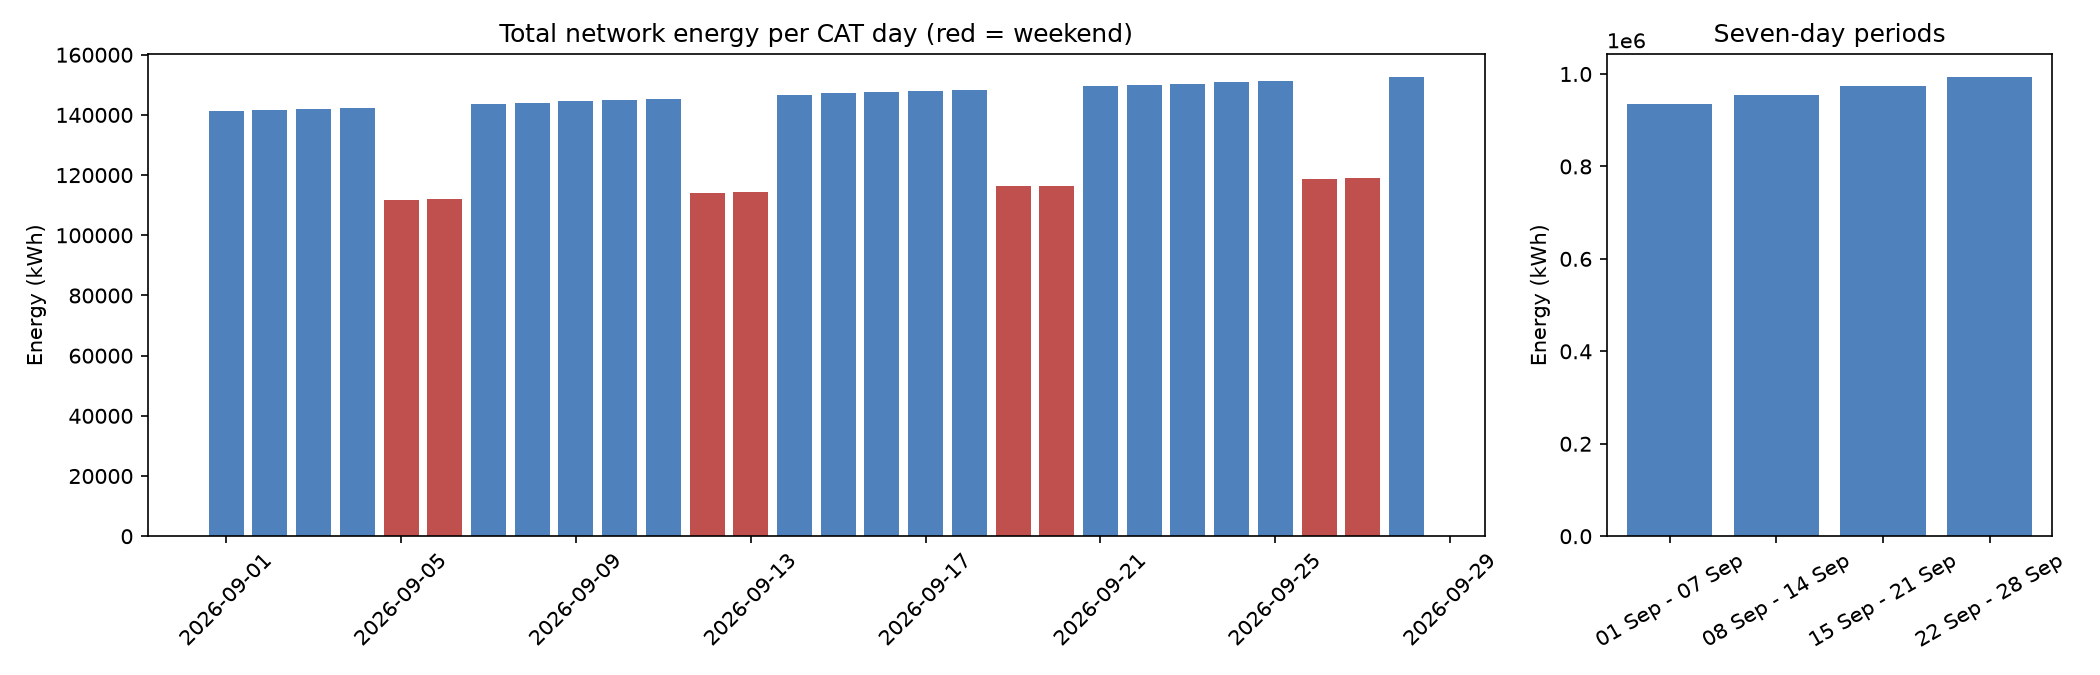
\includegraphics[width=\linewidth]{figures/s5_1_daily_weekly_energy.png}
\caption{Total network energy per CAT day (weekends in red) and per seven-day period.}
\end{figure}

\begin{table}[H]\centering\small
\begin{tabular}{lrr}\toprule
Seven-day period & Energy (kWh) & Change\\\midrule
1--7 Sep & 934,199.1 & --\\
8--14 Sep & 953,715.0 & +2.1\,\%\\
15--21 Sep & 973,230.0 & +2.0\,\%\\
22--28 Sep & 992,560.3 & +2.0\,\%\\\bottomrule
\end{tabular}\hspace{1cm}
\begin{tabular}{lr}\toprule
15-minute interval (CAT) & Network kW\\\midrule
Mon 28 Sep 13:00 & 7,993.7\\
Mon 28 Sep 12:45 & 7,943.9\\
Mon 28 Sep 13:15 & 7,943.6\\\bottomrule
\end{tabular}
\caption{Weekly energy totals (left) and the three highest demand intervals (right).}
\end{table}

\begin{figure}[H]\centering
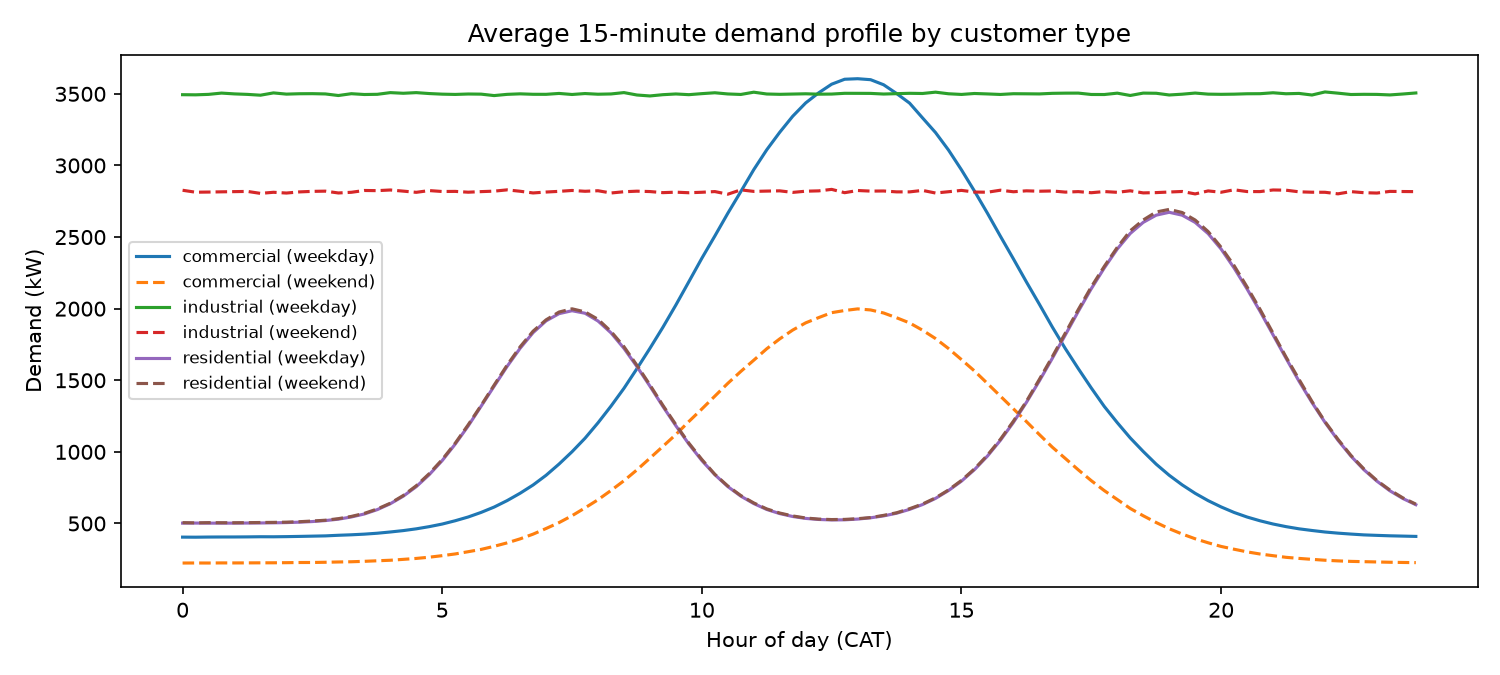
\includegraphics[width=0.85\linewidth]{figures/s5_1_daily_profile.png}
\caption{Average 15-minute demand profile by customer type and day type.}
\end{figure}

\paragraph{Patterns.}
\begin{itemize}
\item Industrial meters provide a large, almost flat base load.
\item Commercial load peaks around 13:00 on business days and falls at weekends.
\item Residential load has a morning peak (about 07:30) and an evening peak (about
19:00).
\end{itemize}
Network demand therefore peaks at weekday midday. The three highest intervals fall on
the last Monday because of the growth trend.

\paragraph{Operational implications.}
\begin{itemize}
\item Capacity must cover a growing weekday midday peak.
\item Maintenance is best scheduled at night or at weekends.
\item Energy procurement needs to grow by about 2\,\% per week.
\end{itemize}

\paragraph{kW versus kWh.}
Kilowatts (kW) measure instantaneous demand, which sizes generation and network
capacity. Kilowatt-hours (kWh) measure energy delivered over time, which drives billing
and procurement. A short, high kW peak can be costly even when its kWh contribution is
small.

\shot{5_1_analysis.png}{Executed analysis and peak-interval results.}

\subsection{Compare regions and customer types}

\begin{table}[H]\centering\small
\begin{tabular}{lrrrr}\toprule
Customer type & Meters & Energy (kWh) & kWh per meter & Share\\\midrule
industrial & 406 & 2,220,672 & 5,469.6 & 57.6\,\%\\
commercial & 1,010 & 825,475 & 817.3 & 21.4\,\%\\
residential & 2,584 & 807,557 & 312.5 & 21.0\,\%\\\bottomrule
\end{tabular}
\caption{Energy by customer type over 28 days.}
\end{table}

\begin{table}[H]\centering\small
\begin{tabular}{lrrrr}\toprule
Region & Meters & Energy (kWh) & kWh per meter & Industrial meters\\\midrule
Region 8 & 400 & 503,475.8 & 1,258.7 & 61\\
Region 5 & 400 & 411,040.4 & 1,027.6 & 48\\
Region 9 & 400 & 400,467.2 & 1,001.2 & 45\\
Region 3 & 400 & 392,376.6 & 980.9 & 46\\
Region 1 & 400 & 383,539.8 & 958.8 & 37\\
Region 2 & 400 & 378,448.9 & 946.1 & 39\\
Region 7 & 400 & 362,288.5 & 905.7 & 35\\
Region 10 & 400 & 351,149.8 & 877.9 & 34\\
Region 6 & 400 & 346,512.8 & 866.3 & 32\\
Region 4 & 400 & 324,404.5 & 811.0 & 29\\\bottomrule
\end{tabular}
\caption{Energy by region over 28 days, with the number of industrial meters.}
\end{table}

\paragraph{Customer types.}
Normalising by meter count removes the effect of group size. An industrial meter still
uses 17.5$\times$ as much energy as a residential one.

\paragraph{Regions.}
Every region has 400 meters, so normalisation does not change the ranking: Region~8
still uses 55\,\% more energy per meter than Region~4. The industrial meter count follows
the same ranking (61 against 29). Regional differences therefore reflect customer mix,
not regional behaviour. Capacity planning should follow the number of industrial
customers, and fair regional comparisons also need normalisation by customer type.

\shot{5_2_groups.png}{Group meter counts and comparison results.}

\subsection{Assess reporting quality}

\paragraph{Completeness.}
Over the whole network, completeness was 98.993\,\%. Regions ranged from 98.969\,\%
(Region~6) to 99.013\,\% (Region~8), a spread of only 0.04 points. Losses are random,
not a regional communication fault.

\begin{table}[H]\centering\small
\begin{tabular}{lrr}\toprule
Energy for 21 September & kWh & Readings\\\midrule
Arrivals by 22 Sep 00:00 & 149,400.54 & 379,505\\
All arrivals & 149,552.72 & 380,036\\
Difference & 152.18 (0.102\,\% of final) & 531\\\bottomrule
\end{tabular}
\caption{Effect of delayed arrivals on a daily total.}
\end{table}

\paragraph{Effect of delayed and missing readings.}
\begin{itemize}
\item \textbf{Delayed readings.} All 531 late readings came from the last three hours
of the day. A report produced at midnight understates the evening peak, but the data
arrives later, so daily totals should be marked provisional and finalised after about
03:00.
\item \textbf{Missing readings.} The roughly 1\,\% of readings that never arrive is
never recovered, so totals are permanently about 1\,\% low unless gaps are estimated
explicitly.
\end{itemize}

\shot{5_3_completeness.png}{Completeness calculation and the two daily totals.}

\subsection{Investigate abnormal consumption}

\paragraph{Rule.}
The rule was fixed before the labels were consulted. For each reading:
\begin{itemize}
\item the \textit{expected} power is the median \texttt{power\_kw} of the same meter, in
the same 15-minute slot of the CAT day and the same day type (weekday or weekend), over
all 28 days;
\item the reading is flagged when $\text{power}/\text{expected} \ge 2.0$ (spike) or
$\le 0.4$ (drop).
\end{itemize}

\paragraph{Reasons for this rule.}
\begin{itemize}
\item Each customer type has its own daily shape, and commercial load falls at weekends.
Comparing like with like removes the normal pattern.
\item The median is not moved by a single abnormal day.
\item Normal noise is about $\pm$15\,\% plus at most 8\,\% trend, so normal ratios stay
within roughly 0.8--1.25. The 2.0 and 0.4 limits leave a wide margin.
\end{itemize}
The flags were written to the table \texttt{anomaly\_flags} (\texttt{meter\_id},
\texttt{event\_time}). Only then did the program call \texttt{anomaly\_events()}.

\begin{table}[H]\centering\small
\begin{tabular}{lr}\toprule
Measure & Value\\\midrule
Flags raised (spike / drop) & 474 (236 / 238)\\
Injected events detected & \textbf{40 / 40}\\
Injected events missed & 0\\
False flags & 0 (0\,\% of 10,643,261 readings outside injected intervals)\\
Percentage of meters affected by false flags & 0\,\% (0 of 4,000)\\\bottomrule
\end{tabular}
\caption{Anomaly detection evaluated against the 40 supplied events.}
\end{table}

\paragraph{Interpretation.}
The 474 flags cover every observed reading inside the 40 three-hour windows (480
planned, 6 missing). The injected factors of 2.8$\times$ and 0.03$\times$ lie far
outside normal variation, which is why nothing was missed and nothing was falsely
flagged. In real data:
\begin{itemize}
\item events would be missed when changes are milder, when they fall inside missing
readings, or when an anomaly recurs often enough to shift the median;
\item false alarms would come from holidays, outages or genuine changes in a
customer's equipment.
\end{itemize}
Lowering the thresholds trades more detections for more false alarms.

\shot{5_4_detection.png}{Executed detection, flagged readings and comparison with the injected events.}

\subsection{Management recommendation}
\begin{tcolorbox}[colback=white, colframe=black!25, boxrule=0.5pt, arc=0pt]
\small
\textbf{To:} Operations and IT management \quad \textbf{Re:} Smart-meter analytics, September 2026

\medskip
\textbf{Operations.} Network demand peaks on weekday middays (about 13:00), driven by
commercial load on top of a large, flat industrial base. The highest 15-minute demand
was 7,994\,kW on Monday 28 September, and weekly energy grew steadily by about 2\,\%
per week (934 to 993\,MWh). Capacity plans should therefore be based on the weekday
midday kW peak, adjusted for this growth. Maintenance should be scheduled at weekends,
when consumption is about 21\,\% lower. Industrial meters (10\,\% of meters) use
58\,\% of the energy, and they explain why Region~8 uses 55\,\% more per meter than
Region~4. Key-account monitoring for industrial customers would give the largest
benefit per meter. Our anomaly rule, which compares each reading with the same meter's
usual load at that time and day type, found all 40 test events with no false alarms.
We recommend running it daily and investigating flags within 24 hours.

\medskip
\textbf{Data quality and reporting.} About 1\,\% of readings never arrive and 2\,\%
arrive up to three hours late. Daily reports produced at midnight understate
consumption (by 152\,kWh, 0.1\,\%, on 21 September). Gaps must never be treated as zero
use. Daily figures should be published as provisional at midnight and finalised after
03:00, with completeness (currently 98.99\,\%, uniform across regions) reported
alongside.

\medskip
\textbf{Storage and dashboards.} Keep raw readings in TimescaleDB hypertables with
one-day chunks, compressed after 48 hours with meter segmentation. This cuts storage by
65\,\% (1,417 to 502\,MB per month of data). Full-history queries become 66--82\,\%
faster and single-meter lookups stay at about 2\,ms. Serve dashboards from continuous
aggregates: a full refresh takes 0.54\,s instead of 3.6\,s (6.7$\times$ faster), for
18\,MB of extra storage and a 15-minute refresh job.

\medskip
\textbf{Forecasting.} Adopt the Ridge regression day-ahead forecast. On the test week
its error was 4.56\,kWh MAE per region-hour (RMSE 5.79\,kWh), against 42.7\,kWh (RMSE
79.4\,kWh) for the ``same as yesterday'' baseline, an 89\,\% reduction. It is especially
better around weekends: on Monday 28 September the baseline under-forecast the regional
peak by up to 270\,kWh, against at most 18\,kWh for the model. Retrain weekly, add
holiday information, and run the forecast after late readings have arrived.
\end{tcolorbox}

% ================================================================== 6
\section{Create and investigate continuous aggregates}

\subsection{Create the three aggregate views}
\texttt{sql/10\_caggs.sql} creates three views over \texttt{energy\_readings}, all
\texttt{WITH NO DATA} and with \texttt{timescaledb.materialized\_only = true}:
\begin{itemize}
\item \texttt{cagg\_energy\_15m\_region}: 15-minute bucket $\times$ region;
\item \texttt{cagg\_energy\_hour\_region}: CAT hour $\times$ region;
\item \texttt{cagg\_energy\_day\_meter}: CAT day $\times$ \texttt{meter\_id}, using
\texttt{time\_bucket('1 day', \ldots, 'Africa/Kigali')}.
\end{itemize}
The two regional views use an inner join to \texttt{meters} on \texttt{meter\_id}.
Each view stores the bucket, its key, the sum of energy, the sum of power and the
reading count.

\texttt{src/s6\_1\_refresh.py} refreshed each view over 1--29 September and measured it
before any policy was added.

\begin{table}[H]\centering\small
\begin{tabular}{lrrrrr}\toprule
View & Rows & Refresh (s) & Data MB & Index MB & Total MB\\\midrule
cagg\_energy\_15m\_region & 26,880 & 15.9 & 2.11 & 2.04 & 4.15\\
cagg\_energy\_hour\_region & 6,720 & 22.2 & 0.64 & 0.59 & 1.23\\
cagg\_energy\_day\_meter & 112,000 & 17.6 & 7.41 & 5.15 & 12.55\\\bottomrule
\end{tabular}
\caption{Initial refresh and materialized size.}
\end{table}

Policies were then added to all three views: a three-day lookback, a one-hour end
offset and a 15-minute schedule. Their window is relative to the database clock, which
is now in October, so they never refresh September. That is why the manual refresh was
required.

\shot{6_1_views.png}{View definitions and sample populated rows.}
\shot{6_1_refresh.png}{Storage and initial refresh measurements, policy settings and job status.}

\subsection{Test freshness and delayed arrivals}
\texttt{src/s6\_2\_freshness.py} uses its own test hypertable and an hourly aggregate
(no data at creation, real-time off, no policy).

\begin{itemize}
\item \textbf{Test time:} 3 October 10:42 CAT.
\item \textbf{Hours used:} $H$ = 3 October 09:00, so the older hour is 1 October 09:00.
\item \textbf{Inserts:} 1 October 09:10 (1\,kWh), 1 October 09:25 (0.5\,kWh) and
3 October 09:10 (2\,kWh).
\end{itemize}

\begin{table}[H]\centering\small
\begin{tabularx}{\linewidth}{Xllll}\toprule
Stage & Raw older & Raw $H$ & Aggregate older & Aggregate $H$\\\midrule
1. 1\,kWh inserted, older hour refreshed, real-time off & 1.0, 1 row & -- & 1.0, 1 row & no bucket\\
2. +0.5\,kWh older, +2\,kWh $H$, no refresh, real-time off & 1.5, 2 rows & 2.0, 1 row & 1.0, 1 row & no bucket\\
3. Real-time on, no refresh & 1.5, 2 rows & 2.0, 1 row & 1.0, 1 row & 2.0, 1 row\\
4. Both hours refreshed & 1.5, 2 rows & 2.0, 1 row & \textbf{1.5, 2 rows} & \textbf{2.0, 1 row}\\\bottomrule
\end{tabularx}
\caption{Freshness test results (kWh, rows).}
\end{table}

\paragraph{What became visible at each stage.}
\begin{itemize}
\item \textbf{Stage 1.} Only the refreshed older hour is materialized.
\item \textbf{Stage 2.} The new rows exist in the raw table but not in the
materialization. The older hour is stale at 1\,kWh, and no bucket exists for $H$; an
absent bucket is not a zero reading.
\item \textbf{Stage 3.} Real-time aggregation combines materialized data below the
watermark (1 October 10:00) with raw data above it. $H$ therefore appears with
2\,kWh, but the late insert into the older hour, which is below the watermark, stays
invisible until a refresh processes its invalidation.
\item \textbf{Stage 4.} The manual refresh brings both hours up to date and moves the
watermark to 3 October 10:00.
\end{itemize}

\paragraph{What the Section~6.1 policy could refresh.}
At 10:42 the policy's window was [30 September 10:42, 3 October 09:42), and only whole
buckets inside the window are refreshed.
\begin{itemize}
\item The older hour \textbf{could} be refreshed.
\item Hour $H$ (09:00--10:00) \textbf{could not}: it ends after 09:42, so it becomes
refreshable only after 11:00. Until then it is visible only through real-time
aggregation.
\end{itemize}

\shot{6_2_setup.png}{Test table and view definitions, inserts and real-time settings.}
\shot{6_2_stages.png}{Raw and aggregate results at each stage.}

% ================================================================== 7
\section{Build and compare dashboards}

\subsection{Raw dashboard}
We used Plotly Dash (\texttt{dashboard/app.py}). The Raw dashboard queries
\texttt{energy\_readings} directly and joins \texttt{meters} where needed. Its filters
are a whole-CAT-day date range and a selected meter. It has five panels:
\begin{itemize}
\item hourly regional energy (kWh);
\item daily network energy (kWh);
\item network energy in the seven-day periods of Section~5.1 (kWh);
\item daily energy of the selected meter (kWh);
\item completeness by region (\%).
\end{itemize}
Every panel is limited to the selected range. The panel queries are kept in
\texttt{dashboard/queries.py}.

\shot{7_1_raw.png}{Running Raw dashboard with all five panels.}

\subsection{Aggregate dashboard}
The Aggregate dashboard has the same panels, layout, filters and date range, but reads
only the continuous aggregates:
\begin{itemize}
\item hourly regional energy comes from \texttt{cagg\_energy\_hour\_region};
\item daily and weekly network energy and the observed completeness counts come from
\texttt{cagg\_energy\_15m\_region}, summing the stored sums and counts;
\item meter history comes from \texttt{cagg\_energy\_day\_meter}.
\end{itemize}
Planned readings are calculated as registered meters (from \texttt{meters}) $\times$
days $\times$ 96.

\shot{7_2_aggregate.png}{Running Aggregate dashboard and its panel query definitions.}

\subsection{Verify matching results}
Both dashboards were set to 22 September 00:00 -- 29 September 00:00 (exclusive),
with all regions and meter 1000000000. \texttt{src/s7\_3\_verify.py} matched the data
behind each panel by its keys.

\begin{table}[H]\centering\small
\begin{tabular}{lrcrc}\toprule
Panel & Rows compared & Keys and counts identical & Max.\ abs.\ difference & Result\\\midrule
Hourly regional energy & 1,680 & yes & 0.000000 kWh & pass\\
Daily network energy & 7 & yes & 0.000000 kWh & pass\\
Seven-day network energy & 1 & yes & 0.000000 kWh & pass\\
Selected meter, daily & 7 & yes & 0.000000 kWh & pass\\
Completeness by region & 10 & yes & 0.000000 pp & pass\\\bottomrule
\end{tabular}
\caption{Raw against Aggregate panel data (limits: 0.001\,kWh and 0.000001 percentage points).}
\end{table}

\shot{7_3_paired.png}{Paired dashboard outputs and numerical checks for all five panels.}

\subsection{Measure performance and judge the tradeoff}

\paragraph{Procedure.}
\begin{itemize}
\item All background jobs were paused, and the dashboards have no result caching.
\item In each mode, one warm-up and ten measured refreshes ran automatically in the
same browser, on the same machine and connection.
\item \textbf{Tools:} per-panel query time was measured on the server with Python's
\texttt{time.perf\_counter()}. Whole-dashboard time was measured in the browser with
\texttt{performance.now()}, from the refresh request until all five Plotly graphs had
drawn that refresh.
\end{itemize}

\begin{table}[H]\centering\small
\begin{tabular}{lrrrrrr}\toprule
 & \multicolumn{3}{c}{Raw} & \multicolumn{3}{c}{Aggregate}\\
\cmidrule(lr){2-4}\cmidrule(lr){5-7}
Measure (ms) & median & min & max & median & min & max\\\midrule
Whole dashboard & 3586.7 & 2544.5 & 4594.4 & \textbf{536.0} & 79.1 & 577.7\\
Hourly regional & 1874.6 & 874.1 & 3871.6 & 34.3 & 10.6 & 39.6\\
Daily network & 997.3 & 801.3 & 2167.6 & 14.1 & 8.3 & 28.5\\
Seven-day network & 2297.5 & 977.7 & 3213.6 & 15.7 & 13.1 & 21.6\\
Selected meter & 28.4 & 8.6 & 410.1 & 6.4 & 3.0 & 24.0\\
Completeness & 1265.2 & 534.7 & 2667.4 & 16.0 & 7.1 & 25.8\\\bottomrule
\end{tabular}
\caption{Dashboard refresh timings over ten measured refreshes. Aggregate cost from
Section~6.1: 17.9\,MB of storage (1.3\,\% of the raw table) and 55.7\,s of initial
refresh.}
\end{table}

\paragraph{Judgement.}
The speed gain justifies the extra storage and refresh work:
\begin{itemize}
\item the whole dashboard is 6.7$\times$ faster, and the remaining 0.5\,s is mostly
browser rendering;
\item individual panel queries are 4--150$\times$ faster;
\item in Raw mode the five panels scan up to 2.7 million rows each at the same time and
compete for CPU, and this cost grows with the date range and the number of users.
\end{itemize}
The price is small: 18\,MB of storage, a 15-minute refresh job, and aggregates that may
lag by up to about an hour unless real-time aggregation is enabled. All jobs were
resumed after the measurements.

\shot{7_4_timing.png}{Completed timing results and comparison.}

% ================================================================== 8
\section{Forecast the next day}

\subsection{Prepare chronological data and features}

\paragraph{Dataset.}
\begin{itemize}
\item One row per region and CAT hour, summing the cleaned \texttt{energy\_kwh}: 6,720
rows.
\item Readings per region-hour ranged from 1,562 to 1,597 (1,600 planned).
\item The data was reindexed onto a complete grid, which showed \textbf{no absent
region-hours}. Rows with missing predictors would have been excluded.
\end{itemize}

\paragraph{Splits and forecast origin.}
The data was split by target timestamp, as shown in the second table below. The forecast
origin is 00:00 CAT of the target's day.

\begin{table}[H]\centering\small
\begin{tabular}{llll}\toprule
Feature & Lag (h) & Window & Earliest usable target\\\midrule
lag\_24h (same hour, previous day) & 24 & 1 h & 2 Sep 00:00\\
lag\_48h & 48 & 1 h & 3 Sep 00:00\\
lag\_168h (same hour, previous week) & 168 & 1 h & 8 Sep 00:00\\
prev\_day\_total (previous CAT day) & 24--47 & 24 h & 2 Sep 00:00\\
region, hour of day, day of week & calendar & -- & --\\\bottomrule
\end{tabular}
\caption{Features, all available before the forecast origin.}
\end{table}

\begin{table}[H]\centering\small
\begin{tabular}{lllrr}\toprule
Split & Dates (targets) & Limits & Rows & Usable rows\\\midrule
Training & 1--14 Sep & 8 Sep 00:00 -- 14 Sep 23:00 & 3,360 & 1,680\\
Validation & 15--21 Sep & 15 Sep 00:00 -- 21 Sep 23:00 & 1,680 & 1,680\\
Test & 22--28 Sep & 22 Sep 00:00 -- 28 Sep 23:00 & 1,680 & 1,680\\\bottomrule
\end{tabular}
\caption{Chronological splits.}
\end{table}

\paragraph{Lookback.}
The initial lookback is 168 hours. Of 3,360 training rows, 1,680 were excluded (targets
before 8 September) and 1,680 were retained. The same rows were used for every
configuration. We accepted this loss because the one-week lag and day of week capture
the weekend dip and the Monday recovery.

\paragraph{Leakage check and preprocessing.}
The program checks that every lag source timestamp precedes its forecast origin; the
smallest gap is 1 hour, so all sources do. Scaling and one-hot encoding were fitted on
training rows only.

\shot{8_1_dataset.png}{Dataset preparation, split sizes and dates, feature examples and lag checks.}

\subsection{Evaluate the previous-day baseline}
At 00:00 on each test day, each of the 24 hourly values for each region was predicted
as the same hour on the previous day. This gave 1,680 predictions with
\textbf{MAE 42.71\,kWh} and \textbf{RMSE 79.40\,kWh}.

\shot{8_2_baseline.png}{Baseline run, prediction count, sample predictions and metrics.}

\subsection{Train and evaluate one regression model}
We used Ridge regression. The shared predictors are the three lags, the previous-day
total (standardised) and one-hot encodings of region, hour and day of week.

\begin{table}[H]\centering\small
\begin{tabular}{llrrrr}\toprule
ID & Settings & Train rows & Validation rows & Val.\ MAE (kWh) & Val.\ RMSE (kWh)\\\midrule
R1 & Ridge($\alpha$ = 0.1) & 1,680 & 1,680 & \textbf{4.432} & 5.643\\
R2 & Ridge($\alpha$ = 1) & 1,680 & 1,680 & 4.440 & 5.652\\
R3 & Ridge($\alpha$ = 10) & 1,680 & 1,680 & 4.818 & 6.183\\
R4 & Ridge($\alpha$ = 100) & 1,680 & 1,680 & 7.955 & 11.773\\\bottomrule
\end{tabular}
\caption{Validation comparison. R1 was selected and frozen.}
\end{table}

The selected model was never refitted. It produced the same 1,680 test predictions as
the baseline, using only information available before each origin; earlier completed
test days supply later lag values only.

\shot{8_3_model.png}{Training completion, validation MAE per configuration, selected settings and sample test predictions.}

\subsection{Judge forecast usefulness}
Error is defined as predicted minus actual, in kWh.

\begin{table}[H]\centering\small
\begin{tabular}{lrrrrr}\toprule
Region & Baseline MAE & Model MAE & Baseline RMSE & Model RMSE & MAE gain\\\midrule
\textbf{All (1,680)} & \textbf{42.71} & \textbf{4.56} & \textbf{79.40} & \textbf{5.79} & \textbf{89.3\,\%}\\
Region 1 & 44.87 & 4.69 & 83.70 & 5.87 & 89.5\,\%\\
Region 2 & 41.63 & 4.53 & 76.81 & 5.65 & 89.1\,\%\\
Region 3 & 42.75 & 4.26 & 77.61 & 5.56 & 90.0\,\%\\
Region 4 & 34.86 & 4.06 & 64.23 & 5.12 & 88.4\,\%\\
Region 5 & 44.40 & 5.23 & 81.08 & 6.61 & 88.2\,\%\\
Region 6 & 39.43 & 3.72 & 74.77 & 4.69 & 90.6\,\%\\
Region 7 & 39.69 & 4.39 & 73.94 & 5.74 & 88.9\,\%\\
Region 8 & 55.97 & 5.82 & 102.06 & 7.17 & 89.6\,\%\\
Region 9 & 43.77 & 4.67 & 80.18 & 5.79 & 89.3\,\%\\
Region 10 & 39.72 & 4.23 & 74.28 & 5.30 & 89.4\,\%\\\bottomrule
\end{tabular}
\caption{Test metrics in kWh, overall and by region.}
\end{table}

\begin{figure}[H]\centering
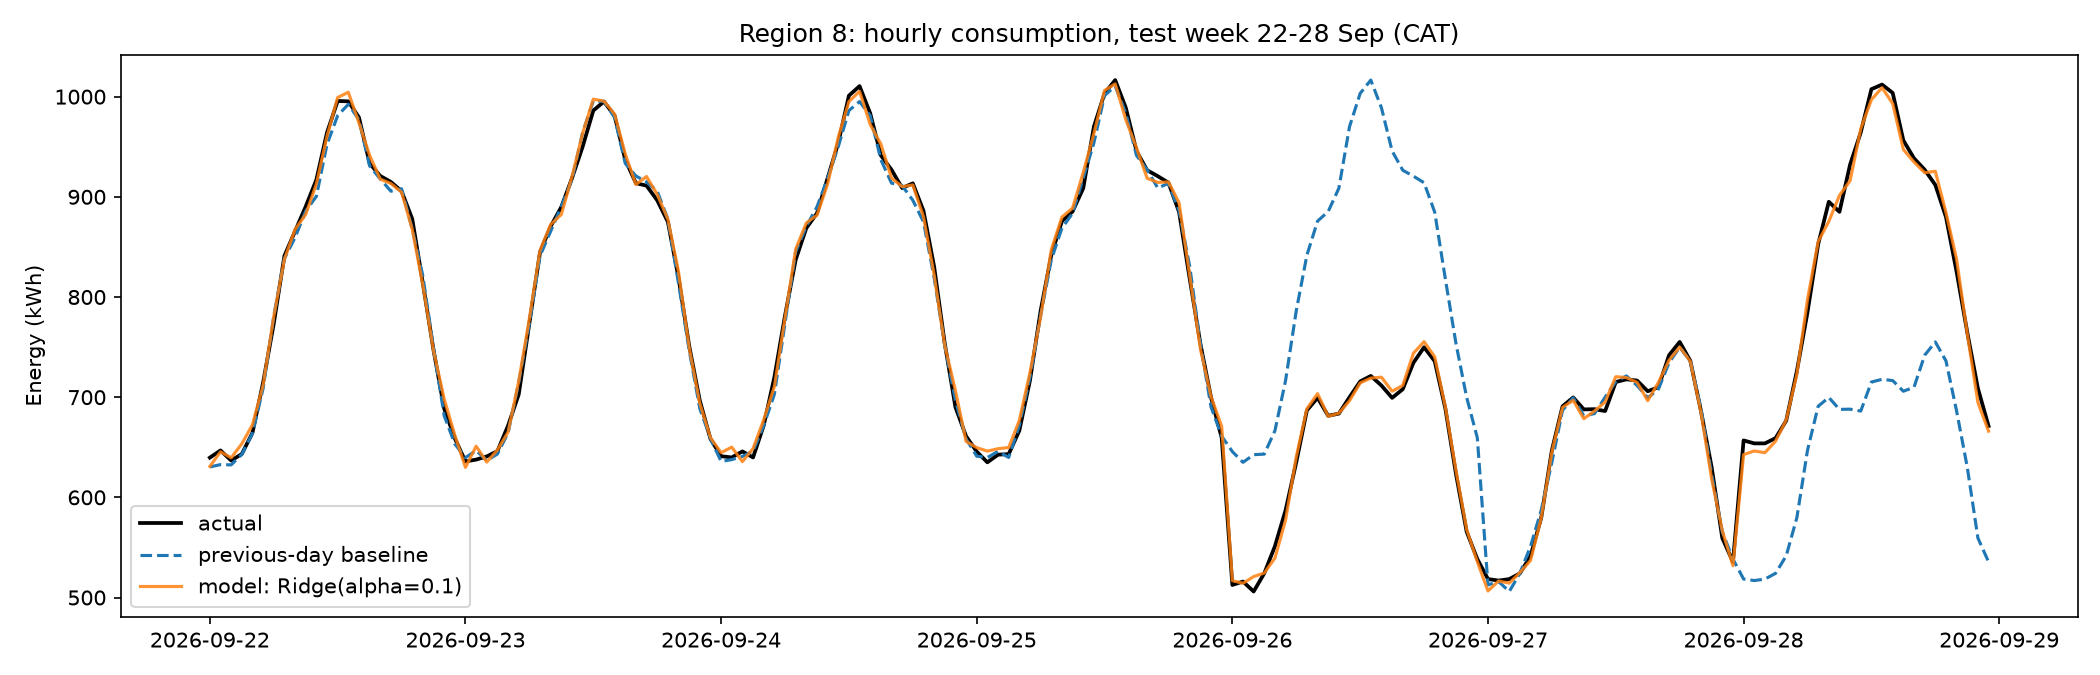
\includegraphics[width=\linewidth]{figures/s8_forecast_region.png}
\caption{Region 8: actual, baseline and model hourly consumption over the seven test days.}
\end{figure}

\begin{table}[H]\centering\small
\begin{tabular}{llrrrrr}\toprule
Region & Peak hour (CAT) & Actual & Baseline & Abs.\ err. & Model & Abs.\ err.\\\midrule
Region 1 & 28 Sep 13:00 & 835.61 & 565.27 & 270.34 & 826.48 & 9.13\\
Region 2 & 28 Sep 13:00 & 780.13 & 546.91 & 233.21 & 774.24 & 5.89\\
Region 3 & 28 Sep 13:00 & 783.00 & 554.69 & 228.32 & 790.77 & 7.77\\
Region 4 & 28 Sep 18:00 & 659.90 & 561.41 & 98.50 & 655.98 & 3.92\\
Region 5 & 28 Sep 13:00 & 828.23 & 577.36 & 250.87 & 826.20 & 2.03\\
Region 6 & 28 Sep 13:00 & 749.11 & 504.41 & 244.70 & 731.38 & 17.73\\
Region 7 & 25 Sep 13:00 & 751.05 & 736.64 & 14.41 & 743.89 & 7.16\\
Region 8 & 25 Sep 13:00 & 1016.55 & 1010.53 & 6.02 & 1012.73 & 3.82\\
Region 9 & 23 Sep 13:00 & 808.96 & 796.89 & 12.07 & 804.44 & 4.52\\
Region 10 & 28 Sep 13:00 & 743.03 & 502.33 & 240.71 & 735.07 & 7.96\\\bottomrule
\end{tabular}
\caption{Highest actual test hour per region (kWh); ties are broken by the earliest time.}
\end{table}

\paragraph{Does the model improve on the baseline?}
Yes. The model improves on the baseline in every region, reducing MAE by about 89\,\%.
On ordinary weekdays the two methods are similar (MAE about 5\,kWh, under 1\,\% of a
typical hourly value). The gain comes almost entirely from weekday--weekend
transitions, where ``yesterday'' is the wrong comparison:
\begin{itemize}
\item the baseline's MAE was 135.7\,kWh on Saturday 26 September and 139.5\,kWh on
Monday 28 September;
\item the model's MAE was 3.6 and 4.9\,kWh on those days.
\end{itemize}

\paragraph{Peak errors and usefulness for planning.}
The baseline under-forecast the Monday 13:00 peak by up to 270\,kWh (32\,\%), which is
the most dangerous error for capacity planning. The model's peak errors were
2--18\,kWh (under 2.5\,\%), which is useful for day-ahead scheduling and procurement.

\paragraph{Limitations.}
\begin{itemize}
\item The targets are observed totals that already miss about 1\,\% of readings, so the
model forecasts recorded rather than true consumption.
\item There was only one usable training week, and no holidays or weather data.
\item In live use, the lags for the last hours before midnight would be incomplete
because about 2\,\% of readings arrive up to three hours late (Section~5.3). The
forecast should therefore run after about 03:00 or correct for provisional data.
\end{itemize}

\shot{8_4_metrics.png}{Metric comparison, peak-hour errors and forecast plot.}

% ================================================================== 9
\section{Reproducibility and contributions}

\subsection{Code and repository}
The repository (\repourl) and the submitted ZIP contain the same files:
\begin{itemize}
\item the unchanged generator;
\item the capture, MQTT and ingestion programs (\texttt{src/});
\item the SQL files (\texttt{sql/00}--\texttt{10});
\item the benchmark, analysis and model code;
\item the dashboard source and panel queries (\texttt{dashboard/});
\item the recorded timings, validation comparison and environment details
(\texttt{results/});
\item a README with the execution order and commands.
\end{itemize}
The 1.16\,GB CSV is not committed. \texttt{src/s2\_1\_capture\_load.py} regenerates
and reloads it. Passwords appear only as placeholders in \texttt{.env.example}.

\shot{9_2_pilot.png}{README pilot instructions run successfully: all four counts equal 2,000.}

\subsection{Contributions}
\begin{table}[H]\centering\small
\begin{tabularx}{\linewidth}{llX}\toprule
Student ID & Name & Contributions\\\midrule
101406 & Pacifique Mashami & Environment setup, MQTT pilot and full ingestion pipeline (Sections 1--2), repository and README\\
101368 & Prince Murenzi & Chunk-interval and compression benchmarks (Sections 3--4), continuous aggregates and freshness test (Section 6)\\
101371 & Delice Sebaganwa Shami & Demand, regional, quality and anomaly analysis (Section 5), dashboards (Section 7), forecasting (Section 8)\\\bottomrule
\end{tabularx}
\caption{Group members and individual contributions. All members reviewed the full
report and can explain every section.}
\end{table}

\end{document}
